\hypertarget{ux6ce8ux610fux529bux673aux5236ux4e0etransformer}{%
\chapter{注意力机制与Transformer}\label{ux6ce8ux610fux529bux673aux5236ux4e0etransformer}}

\hypertarget{ux6ce8ux610fux529bux673aux5236ux7684ux6838ux5fc3ux539fux7406}{%
\section{注意力机制的核心原理}\label{ux6ce8ux610fux529bux673aux5236ux7684ux6838ux5fc3ux539fux7406}}

\hypertarget{ux4e00ux4f20ux7edfux5e8fux5217ux6570ux636eux5904ux7406ux65b9ux6cd5ux5b58ux5728ux7684ux95eeux9898ux548cux751fux7269ux5b66ux6ce8ux610fux529bux7684ux542fux53d1}{%
\subsection{一、传统序列数据处理方法存在的问题和生物学注意力的启发}\label{ux4e00ux4f20ux7edfux5e8fux5217ux6570ux636eux5904ux7406ux65b9ux6cd5ux5b58ux5728ux7684ux95eeux9898ux548cux751fux7269ux5b66ux6ce8ux610fux529bux7684ux542fux53d1}}

在基于注意力机制的Transformer诞生前，处理序列数据往往使用RNN。它维护一个全局上下文向量，称为隐状态 \(h\)。每次输入一个词元 \(x_t\)，就对 \(h\) 进行更新，把它的信息融合入 \(h\) 中（即将 \(h\) 原有的信息和 \(x_t\) 带来的信息组合）。最后，基于这个全局上下文向量给出输出。但这样产生了两个问题：首先，模型只能一个个依次处理数据，对于长上下文依赖关系（比如文章结尾和开头的呼应）处理效果不佳，受距离较近的噪声影响则偏大，这个问题即便引入门控机制也只是略有缓解；其次，一个向量能容纳的信息量太低，难以表征全局上下文的丰富关系。

针对这些问题，研究人员们开始思考，能否保存每个时间步 \(t\) 输入的向量 \(x_1,\ldots,x_t,\ldots\)，从而将这些信息更灵活地聚合起来呢？

2017年，Google发表论文《Attention is All You Need》。该论文开创性地将注意力机制运用于模型架构中。它采取了``选择性聚焦''的方法，模仿人类的选择性注意力，即保留上下文地所有信息，并在大量的信息中，由模型自主有选择地聚焦于最关键的部分，而忽略其他不重要的信息。例如：人的面前有红色的咖啡杯，也有一些报纸、论文、书。在非自主性的情况下，我们的视觉系统往往被红色的咖啡杯吸引；而我们也可以自主性地、有意识地决定去读书，把注意力放在书上。

\hypertarget{ux4e8cux6ce8ux610fux529bux673aux5236ux7684ux4e09ux4e2aux6838ux5fc3ux7ec4ux4ef6}{%
\subsection{二、注意力机制的三个核心组件}\label{ux4e8cux6ce8ux610fux529bux673aux5236ux7684ux4e09ux4e2aux6838ux5fc3ux7ec4ux4ef6}}

注意力机制将这个生物学过程抽象为三个核心组件，这也是理解其原理的关键：

\begin{enumerate}
\def\labelenumi{\arabic{enumi}.}
\tightlist
\item
  查询 -~Query
\end{enumerate}

对应例子：你想``读书''的这个主观意愿或任务目标。

核心原理：Query~是自主性的、任务驱动的。它代表``我当前想寻找什么？''。在模型中，Query~通常是与当前任务最相关的向量，比如在生成一个token时，我们不仅需要其上一个token的信息，也需要更多的上下文，于是我们根据这个token的信息，去前文查找需要补充的更多信息。

\begin{enumerate}
\def\labelenumi{\arabic{enumi}.}
\setcounter{enumi}{1}
\tightlist
\item
  键 -~Key
\end{enumerate}

对应例子：每个物品的突出特征。比如咖啡杯的``红色''，报纸、论文、书的``文字内容''。

核心原理：Key~是非自主性的、数据本身的提示。它就像是每个信息的``标签''或``标识符''，用于与~Query~进行匹配。系统通过比较~Query~和所有~Key~的相似度，来决定应该关注哪些信息。

\begin{enumerate}
\def\labelenumi{\arabic{enumi}.}
\setcounter{enumi}{2}
\tightlist
\item
  值 -~Value
\end{enumerate}

对应例子：物品本身。咖啡杯这个实体、书中的具体文字内容。

核心原理：Value~是最终被提取的感官输入或信息本身。注意力机制的目的不是选择~Key，而是选择~Key~所对应的~Value。我们根据~Query~和~Key~的匹配结果，来对所有的~Value~进行加权汇总，在大语言模型中，这就意味着完成了上文信息的聚合。

\hypertarget{ux4e09ux6ce8ux610fux529bux673aux5236ux7684ux5de5ux4f5cux6d41ux7a0bux57faux4e8eux4f8bux5b50}{%
\subsection{三、注意力机制的工作流程（基于例子）}\label{ux4e09ux6ce8ux610fux529bux673aux5236ux7684ux5de5ux4f5cux6d41ux7a0bux57faux4e8eux4f8bux5b50}}

现在，我们用这三个组件来还原整个过程：

\begin{enumerate}
\def\labelenumi{\arabic{enumi}.}
\item
  场景设定（输入信息）：环境中有五个物品（五个信息源），每个物品都有自己的 Key（突出特征：颜色、形状等）和 Value（物品本身的内容）。
\item
  非自主性注意力（没有明确 Query 时）：此时，没有一个强烈的``主观意愿''（Query）。系统会倾向于关注那些 Key 最突出的信息。比如，Key 为``红色''的咖啡杯，其视觉显著性远高于其他黑白 Key 的物品。因此，注意力权重自然地偏向了咖啡杯，其对应的 Value 被放大。
\item
  自主性注意力（引入 Query 时）：你产生了``想读书''的意愿，这就是 Query。
\item
  匹配阶段：系统将这个 Query（``想读书''）与环境中所有物品的 Key（报纸的``新闻''、论文的``研究''、书的``文学''）进行相似度比较。计算权重：Query 与``书''的 Key 匹配度最高。因此，``书''这个 Value 被赋予最高的注意力权重。
\item
  汇聚阶段：系统根据计算出的权重，对所有 Value（报纸内容、论文内容、书的内容等）进行加权求和。由于书的权重接近1，其他权重接近0，最终输出的信息几乎完全来自于``书''这个 Value。
\end{enumerate}

总的来说，注意力机制是一个资源分配方案。它通过一个自主性的查询，与一系列非自主性的键进行相似度匹配，从而计算出注意力权重，并利用这些权重对对应的值进行加权求和，最终得到一个聚焦于关键信息的输出。

如果 \(W_Q,W_K,W_V\) 都和相同的 \(X\) 输入相乘，称为自注意力。

\hypertarget{ux56dbux4e0eux5168ux8fdeux63a5ux5c42ux7684ux533aux522b}{%
\subsection{四、与全连接层的区别}\label{ux56dbux4e0eux5168ux8fdeux63a5ux5c42ux7684ux533aux522b}}

全连接层的输出是``按权重对输入加权''，但是在训练完成后，输出的第 \(i\) 个对各个输入的权重是固定的，比较死板，不能很好处理``这个样本中第三个词是关键，下个样本中第二个词是关键''地问题。而在注意力机制中，有三个权重矩阵 \(W_Q,W_K,W_V\)，事实上输入被与不同权重矩阵相乘，分别变为``需要查询什么''``被用于查询的标签''``被查询到的内容''，输出事实上是``按相似度对值加权''。相似度由输入和权重通过相乘等变换得到，可以根据当前任务特征，动态地给不同词分配不同注意力权重，使得模型能聚焦于关键信息；值也由输入经过权重变换得到，更加灵活。

相比而言，全连接层/汇聚层对所有输入信息一视同仁，或者只基于数据的固有属性（非自主性提示）进行处理。注意力机制引入了一个动态的、与当前任务相关的~Query（自主性提示），使得模型能够根据上下文和当前目标，动态地、有选择地关注输入的不同部分。

\hypertarget{ux4e94ux591aux5934ux6ce8ux610fux529b}{%
\subsection{五、多头注意力}\label{ux4e94ux591aux5934ux6ce8ux610fux529b}}

一次自注意力计算，像是只从一个角度去理解句子。但显然，词语之间的关系是多维度的。例如，``The cat sat on the mat'' 中，``sat'' 这个词既和主语``cat''有关（谁在坐），也和地点``mat''有关（坐在哪）。多头注意力就是让模型从多个不同的``角度''或``子空间''去理解上下文关系。

在传统的注意力机制中，我们使用一组查询（\(Q\)）、键（\(K\)）和值（\(V\)）来计算注意力。而多头注意力机制通过将 \(Q,K,V\) 矩阵分割成不同部分（在数学上等价为把它们的向量投影到多个不同维度的子空间），然后在这些子空间中分别计算注意力，最后通过矩阵拼接的方式将结果合并起来。这样可以让模型捕捉到多种不同类型的依赖关系。

例如，在语言理解中，不同头可以分别学习：

头1: 语法依赖 关注: 主语-动词, 动词-宾语, 修饰关系

头2: 语义角色 关注: 施事者, 受事者, 工具, 地点

头3: 指代消解 关注: 代词与其指代对象

头4: 篇章结构 关注: 转折, 因果, 并列关系

头5: 词汇语义 关注: 同义词, 反义词, 上下位关系

头6: 位置模式 关注: 相邻词, 固定距离词

头7: 罕见模式 关注: 特殊结构, 成语

头8: 综合平衡 关注: 整体一致性检查

在视觉任务中：

头1: 颜色特征 头2: 纹理特征 头3: 形状特征 头4: 空间关系 头5: 物体部件 头6: 场景上下文 头7: 运动模式 头8: 显著性检测

\hypertarget{ux516dux591aux5934ux6ce8ux610fux529bux5c42ux7684ux6570ux5b66ux8868ux8fbeux6ce8ux610fux8fd9ux662fux4e00ux4e2aux5c42ux800cux4e0dux662fux4e00ux4e2aux7f51ux7edc}{%
\subsection{六、多头注意力层的数学表达（注意：这是一个层，而不是一个网络）}\label{ux516dux591aux5934ux6ce8ux610fux529bux5c42ux7684ux6570ux5b66ux8868ux8fbeux6ce8ux610fux8fd9ux662fux4e00ux4e2aux5c42ux800cux4e0dux662fux4e00ux4e2aux7f51ux7edc}}

\begin{enumerate}
\def\labelenumi{\arabic{enumi}.}
\tightlist
\item
  第一步：Q、K、V的计算
\end{enumerate}

输入向量：假设我们有一个输入序列，每个时间步的向量为 \(x_i\)（维度为 \(d_{\mathrm{model}}\)，也就是该神经网络的输入特征维度，比如一个词所在 embedding 空间的维度）。

投影矩阵：\(W_Q,W_K,W_V\)（维度为 \(d_{\mathrm{model}}\times d_k\)、\(d_{\mathrm{model}}\times d_k\)、\(d_{\mathrm{model}}\times d_v\)，在有 \(h\) 个头的多头注意力中，通常 \(d_k=d_v=d_{\mathrm{model}}/h\)，也就是说多个头共用）。

相乘操作：

\[
\begin{aligned}
Q_i &= x_i W_Q,\\
K_i &= x_i W_K,\\
V_i &= x_i W_V.
\end{aligned}
\]

以第一条式子为例，如果把这视为一层变换，嵌入向量 \(x_i\) 视为输入，查询向量 \(Q_i\) 视为输出，那么 \(W_Q\) 实际上就表示一种线性变换，将 \(d_{\mathrm{model}}\) 维的输入通过``全连接''转变为 \(d_k\) 维的查询向量输出。从线性代数视角分析，\(W_Q\) 的每一行表示查询空间的一个基向量，它的第 \(j\) 行和 \(x_i\) 的第 \(j\) 列相乘。

实际上，为了计算效率，我们通常用矩阵乘法同时计算所有 \(i\)：\(Q=XW_Q\)，其中 \(X\) 是输入矩阵，每一行是一个 \(x_i\)。

下面还有一个例子（尚未进行多头的切分），可以看出 \texttt{W\_Q} 的``特征重组''作用。

假设输入矩阵 \texttt{X} 简化为 3 个词元，它们分别代表``猫''``追逐''``老鼠''，并用少量特征位示意如下：

\begin{itemize}
\tightlist
\item
  \texttt{x\_1\ =\ {[}0.8,\ 0.9,\ 0.7,\ ...{]}}
\item
  \texttt{x\_2\ =\ {[}0.6,\ 0.2,\ 0.9,\ ...{]}}
\item
  \texttt{x\_3\ =\ {[}0.7,\ 0.8,\ 0.3,\ ...{]}}
\end{itemize}

投影矩阵 \texttt{W\_Q} 的前几列可以理解为不同的查询特征：

\begin{itemize}
\tightlist
\item
  第 1 列：主语检测
\item
  第 2 列：动词检测
\item
  第 3 列：宾语检测
\item
  \texttt{...}
\end{itemize}

示意性地，可以写成：

\begin{verbatim}
          列1(主语检测)   列2(动词检测)   列3(宾语检测)   ...
特征1       0.9             0.1             0.2        ...
特征2       0.8             0.7             0.6        ...
特征3       0.1             0.9             0.1        ...
...
\end{verbatim}

于是，\texttt{Q{[}0,1{]}} 可以近似看成：

\[
Q[0,1] = 0.8 \times 0.1 + 0.9 \times 0.7 + 0.7 \times 0.9 + \cdots = 0.08 + 0.63 + 0.63 + \cdots \approx 1.34
\]

对于多头注意力，把维度更多的 \texttt{d\_model} 维输入变成维度更少的 \texttt{d\_k} 维输出，背后是``特征分解''：每个 token 的特征向量（即 \texttt{d\_model} 维输入）包含了各种特征。在多头注意力中，我们先通过乘 \texttt{W\_Q} 进行特征重组，随后把不同方面的特征交给不同的头处理。在这个过程中，每个头会对不同原特征赋予不同关注度，这些差异会体现在 \texttt{W\_Q} 的权重里，但并不意味着其他特征完全不起作用。随后在注意力计算里，每个注意力头再围绕一个方面的特征与其他 token 进行交互。

有时这三步计算还会加偏置，以 \(Q\) 为例，\(Q=xW_Q+b\)，\(b\) 的每一个元素和 \(W_Q\) 的一列对应。也可以把它理解为：\(Q\) 的第 \(j\) 列等于 \(xW_Q\) 的第 \(j\) 列加上偏置 \(b_j\)。例如，\(b_1\) 表示查询特征1的基础偏置（如上面例子中``主语查询''的基础倾向），\(b_2\) 表示查询特征2的基础偏置（如``动词查询''的基础倾向），\(b_{512}\) 表示查询特征512的基础偏置。

偏置向量可能学习到的模式：

\begin{verbatim}
b_Q = [
  0.05,  # 特征1: 根据本模型的目标倒推，轻微倾向于进行"主语查询"
 -0.10,  # 特征2: 轻微抑制"动词查询"
  0.20,  # 特征3: 较强倾向于"宾语查询"
 -0.05,  # 特征4: 轻微抑制"修饰语查询"
  ...
]
\end{verbatim}

这意味着：即使输入全为零，查询向量也会有特定的模式，模型学习到不同查询特征的``默认激活水平''。

\begin{enumerate}
\def\labelenumi{\arabic{enumi}.}
\setcounter{enumi}{1}
\tightlist
\item
  第二步：（每个头各自）计算注意力权重 \(\alpha=\mathrm{Softmax}\left(QK_i^T/\sqrt{d_k}\right)\)
\end{enumerate}

这步计算每一个查询词元和每一个键词元之间的相似度，并进行归一化，得到相似度矩阵。对于每个注意力头，都各自计算一个这样的相似度矩阵。计算复杂度为 \(O(n^2)\)。

假设我们有一个查询向量 \(q\)（来自 \(Q\)，形状为 \([d_k]\)，代表 \(d_k\) 维空间里的一个词元）和键向量 \(k_i\)（来自 \(K\)，形状为 \([d_k]\)，也代表 \(d_k\) 维空间里的一个词元），那么计算注意力分数时，我们计算 \(q\) 和 \(k_i\) 的点积，可以得到两个向量的相似度分数（然后一般会除以 \(\sqrt{d_k}\) 进行缩放以避免梯度消失）。

当然，实际上要查询的问题并不会只有一个词元，键也是。假设 \(Q\) 的形状为 \([n,d_k]\)（\(n\) 个查询词元向量），\(K\) 的形状为 \([m,d_k]\)（\(m\) 个键词元向量），\(QK^T\) 的结果是一个 \([n,m]\) 的矩阵，其中每个元素 \((i,j)\) 是 \(Q\) 的第 \(i\) 行与 \(K\) 的第 \(j\) 行的点积（向量点积可以表达第 \(i\) 个查询词元与第 \(j\) 个键词元的相似度）。然后，我们对这个矩阵的每一行应用 Softmax 函数（沿着键的维度，即第二维），得到注意力权重矩阵 \(\alpha\)，形状为 \([n,m]\)，使得对于每个查询词元而言，各个键词元规范化后的匹配度之和为1。

\begin{enumerate}
\def\labelenumi{\arabic{enumi}.}
\setcounter{enumi}{2}
\tightlist
\item
  第三步：（每个头各自）与值相乘 \(\mathrm{attn\_output}=\alpha V\)
\end{enumerate}

这里对于每个注意力头，将注意力权重矩阵与值矩阵相乘：\(\alpha\) 的形状为 \([n,m]\)（\(n\) 个查询词元向量，\(m\) 个键词元向量），元素 \((i,j)\) 代表第 \(i\) 个查询词元下，第 \(j\) 个键词元与其的匹配度（选择该键词元的概率）。\(V\) 的形状为 \([m,d_v]\)，储存每个键词元在 \(d_v\) 维（该注意力头的维度）空间中的值。Output 矩阵的第 \(i\) 行和 \(V\) 矩阵的第 \(k\) 列相乘，代表所有键词元的值在第 \(k\) 个维度的分量按照该词元和第 \(i\) 个查询词元的匹配度（也就是第 \(i\) 个查询词元分配在该词上的注意力）加权，得到第 \(i\) 个查询词元查找到的新词元向量的第 \(k\) 维。后续则可以根据该新向量和各向量的相似度用 Softmax 回归等方式输出词元，也可以采取其他采样方式。

\[
o_i = \frac{\sum_{j=1}^{n} \exp\left(\frac{q_i \cdot k_j^T}{\sqrt{d_k}}\right) v_j}{\sum_{j=1}^{n} \exp\left(\frac{q_i \cdot k_j^T}{\sqrt{d_k}}\right)}
\]

上式中，\(\alpha\) 的元素 \((i,j)\) 的值为

\[
\alpha_{i,j} = \frac{\exp\left(\frac{q_i \cdot k_j^T}{\sqrt{d_k}}\right)}{\sum_{t=1}^{n} \exp\left(\frac{q_i \cdot k_t^T}{\sqrt{d_k}}\right)}
\]

它与 \(v_j\) 相乘，再对各个 \(j\) 值相加，就得到 \texttt{attn\_output} 的第 \texttt{i} 行向量 \texttt{o\_i}。

\begin{enumerate}
\def\labelenumi{\arabic{enumi}.}
\setcounter{enumi}{3}
\tightlist
\item
  第四步：（多头拼接后）输出投影 \(\mathrm{output}=\mathrm{attn\_output}W_O\)
\end{enumerate}

在注意力机制中，输出投影是将多头注意力的合并输出通过一个线性变换，以对各个低级特征进行整合，获得更高级的特征，或者所需的各种结果，起到将各个头的结果综合进行决策的效果。\texttt{attn\_output} 的形状为 \texttt{{[}seq\_len,d\_model{]}}，\(W_O\) 的形状为 \([d_{\mathrm{model}},d_{\mathrm{model}}]\)，第 \(i\) 列表示新的第 \(i\) 个特征分别取旧的各个特征的比率。这样最终可以得到一个 \([\mathrm{seq\_len},d_{\mathrm{model}}]\) 维、富含上下文表示的矩阵，即一个和输入等长的序列。如何运用取决于任务，后面Transformer完整架构会介绍。

例如：

\begin{verbatim}
W_O = [
        新特征0  新特征1  新特征2  新特征3
  [0.9,    0.1,    0.2,    0.3],    # 老特征0（语法特征）
  [0.1,    0.8,    0.3,    0.2],    # 老特征1（语义特征）
  [0.2,    0.1,    0.7,    0.4],    # 老特征2（位置特征）
  [0.3,    0.2,    0.1,    0.6]     # 老特征3（上下文特征）
]
\end{verbatim}

现在第一个词元``猫''参与计算，假设其四个特征值为 \(x_1,x_2,x_3,x_4\)（\texttt{attn\_output} 的第一行）。

新特征0: {[}0.9, 0.1, 0.2, 0.3{]} → 主要依赖语法特征，轻微使用其他特征

用途: 生成``语法增强的语义表示''，整合了``猫''作为主语的信息，适合用于句法分析任务。

第一个词元的新特征0（语法增强表示，输出矩阵 \((0,0)\) 位置）：\(0.9x_1+0.1x_2+0.2x_3+0.3x_4\)

列1: {[}0.1, 0.8, 0.1, 0.2{]} → 主要依赖语义特征

用途: 生成``纯语义内容表示''，整合了``猫''的动物语义，适合用于词义理解任务。

第一个词元的新特征1（语义内容表示，输出矩阵 \((0,1)\) 位置）：\(0.1x_1+0.8x_2+0.1x_3+0.2x_4\)

列2: {[}0.2, 0.3, 0.7, 0.1{]} → 主要依赖位置特征

用途: 生成``位置感知的表示''，整合了``猫''在句子中的位置信息，适合用于指代消解任务。

列3: {[}0.3, 0.2, 0.4, 0.6{]} → 平衡使用各种特征

用途: 生成``综合上下文表示''，根据训练任务优化的综合表示，适合用于翻译等综合任务。

另外，若某一行的值显著大于其他行，则表明该模型对这个老特征依赖度较高（比如内容情感分析更依赖语义特征）。

\begin{enumerate}
\def\labelenumi{\arabic{enumi}.}
\setcounter{enumi}{4}
\tightlist
\item
  伪代码举例：
\end{enumerate}

\begin{verbatim}
# 输入: "The cat sat on the mat"
# 翻译: "猫 坐在 垫子 上"
# 当生成"猫"时：

Q = [名词, 动作主体, 主语]  # 解码器的当前状态

# 编码器的Keys:
K = [
    [定冠词, 无实际意义],  # The
    [名词, 动物, 主语],     # cat
    [动词, 过去式],        # sat
    [介词],               # on
    [定冠词, 无实际意义],  # the
    [名词, 物体, 地点]     # mat
]

# 计算相似度：
scores = Q · K^T = [0.1, 0.9, 0.3, 0.1, 0.1, 0.4]  # 与"cat"最相似
weights = softmax(scores / sqrt(d_k)) = [0.05, 0.55, 0.1, 0.05, 0.05, 0.2]

# 加权求和Values得到输出
output = 0.05*V_The + 0.55*V_cat + 0.1*V_sat + ...
# 输出主要包含"猫"的信息，用于生成正确翻译
\end{verbatim}

\begin{enumerate}
\def\labelenumi{\arabic{enumi}.}
\setcounter{enumi}{5}
\tightlist
\item
  权重数量
\end{enumerate}

（1）\(W_Q,W_K,W_V\)：假设输入维度为 \(d_{\mathrm{model}}\)，输出使用多头注意力，头数为 \(h\)，每个头的维度为 \(d_k=d_{\mathrm{model}}/h\)（一般情况下，让输入输出在同样维度的嵌入空间中）。每个头的权重数量为 \(3d_{\mathrm{model}}d_k\)。因为有 \(h\) 个头，所以总权重数量为 \(3d_{\mathrm{model}}d_kh=3d_{\mathrm{model}}(d_{\mathrm{model}}/h)h=3d_{\mathrm{model}}^2\)。有时得到 \(Q,K,V\) 的三重线性变换还会包含偏置，则为 \(3d_{\mathrm{model}}^2+3d_{\mathrm{model}}\)。

（2）\(W_O\)：输入维度为 \(d_kh\)，输出维度为 \(d_{\mathrm{model}}\)。总权重数量为 \(d_{\mathrm{model}}^2\)，有偏置则为 \(d_{\mathrm{model}}^2+d_{\mathrm{model}}\)。

合计：\(4d_{\mathrm{model}}^2(+4d_{\mathrm{model}})\)。

\hypertarget{ux4e03ux4ee3ux7801ux5b9eux73b0}{%
\subsection{七、代码实现}\label{ux4e03ux4ee3ux7801ux5b9eux73b0}}

\begin{verbatim}
import torch
import torch.nn as nn
import math


class MultiHeadAttention(nn.Module):
    def __init__(self, d_model=512, num_heads=8):
        super().__init__()
        self.d_model = d_model
        self.num_heads = num_heads
        self.d_k = d_model // num_heads

        # 投影矩阵
        self.W_q = nn.Linear(d_model, d_model)  # [嵌入维度，查询词元向量的维度]
        self.W_k = nn.Linear(d_model, d_model)
        self.W_v = nn.Linear(d_model, d_model)
        self.W_o = nn.Linear(d_model, d_model)

    def forward(self, X):
        batch_size, seq_len, d_model = X.shape  # [批次样本数，序列长度，嵌入维度]

        # 1. Q,K,V投影
        Q = self.W_q(X)  # [batch, seq_len, d_model]
        K = self.W_k(X)  # [batch, seq_len, d_model]
        V = self.W_v(X)  # [batch, seq_len, d_model]

        # 2. 分割成多头
        # 对于batch中的每一个样本，将seq_len*d_model的矩阵变为seq_len*h*d_k，
        # 再用transpose(1, 2)变成h*seq_len*d_k以便按h拆分。
        Q = Q.view(batch_size, seq_len, self.num_heads, self.d_k).transpose(1, 2)
        K = K.view(batch_size, seq_len, self.num_heads, self.d_k).transpose(1, 2)
        V = V.view(batch_size, seq_len, self.num_heads, self.d_k).transpose(1, 2)

        # 现在形状: [batch, num_heads, seq_len, d_k]
        # 维度1为头索引，维度2为序列位置，维度3为该头学习的不同特征。

        # 3. 每个头计算注意力
        scores = torch.matmul(Q, K.transpose(-2, -1)) / math.sqrt(self.d_k)
        attn_weights = torch.softmax(scores, dim=-1)
        head_outputs = torch.matmul(attn_weights, V)

        # 4. 合并多头，形状变回去
        merged = head_outputs.transpose(1, 2).contiguous().view(
            batch_size, seq_len, d_model
        )

        # 5. 输出投影
        output = self.W_o(merged)
        return output
\end{verbatim}

\hypertarget{ux53c2ux8003ux6587ux732e-66}{%
\subsection{参考文献}\label{ux53c2ux8003ux6587ux732e-66}}

\begin{itemize}
\tightlist
\item
  Vaswani, A., Shazeer, N., Parmar, N., et al.~(2017). \href{https://arxiv.org/abs/1706.03762}{Attention Is All You Need}. NeurIPS 2017.
\end{itemize}

\clearpage

\hypertarget{bahdanauux6ce8ux610fux529b}{%
\section{Bahdanau注意力}\label{bahdanauux6ce8ux610fux529b}}

Bahdanau 注意力将通用的注意力思想巧妙地具体化，以解决当时Seq2Seq模型（如基于RNN的编码器-解码器架构）的一个核心痛点。

在传统的Seq2Seq模型中，编码器需要将整个输入序列（如一个句子）压缩成一个固定长度的上下文向量（Context Vector），然后解码器基于这个单一向量生成输出序列。这种方式存在明显的信息瓶颈（Information Bottleneck）：对于长句子，一个固定大小的向量很难完整保留所有信息，导致模型性能下降，尤其容易丢失序列开头部分的细节 。

Bahdanau 注意力的核心创新在于，它允许解码器在生成每一个输出词时，都能``回顾''编码器所有时间步的隐藏状态，并动态地为它们分配本次生成时的注意力权重，计算专属本次生成的上下文向量。这个过程可以概括为三步：

\begin{enumerate}
\def\labelenumi{\arabic{enumi}.}
\item
  评分：使用一个小型神经网络（通常是单层前馈网络），以解码器上一时间步的隐藏状态作为查询Query（比如翻译句子，Query就是已经翻译好的部分，提出对接下来从原句中找下一个词的``需求''），编码器每一个时间步的隐藏状态（待翻译的原句子的每个词）作为键Key，计算它们之间的相关性分数（对齐分数）。
\item
  加权：将对齐分数通过Softmax函数转化为权重（即注意力分布），这些权重之和为1，代表了模型生成当前输出词时，对输入序列不同部分的``关注''程度。
\item
  生成上下文向量：计算编码器所有隐藏状态（作为值Value，也就是语义空间中的词向量）的加权和，得到当前时间步的上下文向量。这个向量聚焦于当前最相关的输入信息，然后被送入解码器辅助生成当前词。
\end{enumerate}

这种方法的关键优势在于，对齐操作（即确定源语言和目标语言词语间的对应关系）不再是独立预处理步骤，而是在端到端的训练过程中与翻译任务联合学习得到的。

\hypertarget{ux53c2ux8003ux6587ux732e-67}{%
\subsection{参考文献}\label{ux53c2ux8003ux6587ux732e-67}}

\begin{itemize}
\tightlist
\item
  Aston Zhang, Zachary C. Lipton, Mu Li, Alexander J. Smola. (2023). \href{https://zh.d2l.ai/}{《动手学深度学习》}. Cambridge University Press.
\item
  Bahdanau, D., Cho, K., \& Bengio, Y. (2015). \href{https://arxiv.org/abs/1409.0473}{Neural Machine Translation by Jointly Learning to Align and Translate}. ICLR 2015.
\end{itemize}

\clearpage

\hypertarget{transformer}{%
\section{Transformer}\label{transformer}}

Transformer是Google于2017年提出的架构，是目前所有大模型架构的基础。

\begin{figure}[htbp]
\centering
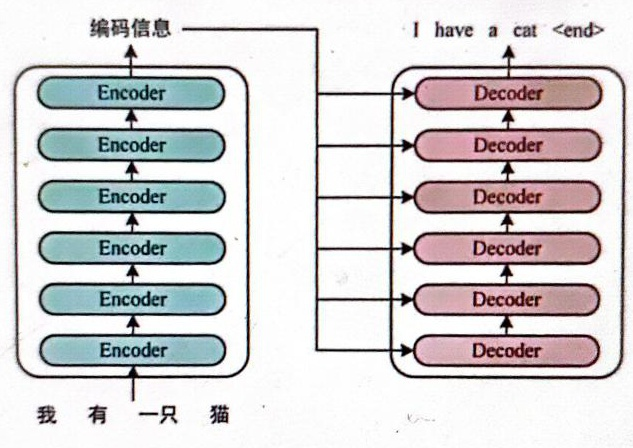
\includegraphics{images/image-0015.jpeg}
\caption{Transformer 的整体结构示意图}
\end{figure}

Transformer 的整体结构：左侧为 Encoder，右侧为 Decoder。

\begin{figure}[htbp]
\centering
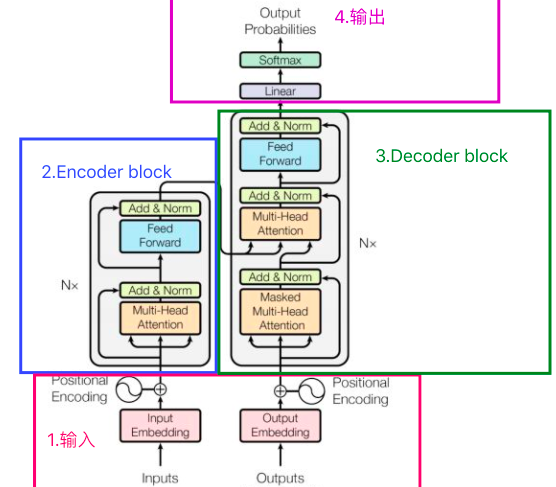
\includegraphics{images/image-0016.png}
\caption{Transformer 模块总览图}
\end{figure}

\hypertarget{ux4e00ux8f93ux5165}{%
\subsection{一、输入}\label{ux4e00ux8f93ux5165}}

\begin{enumerate}
\def\labelenumi{\arabic{enumi}.}
\item
  左下 inputs 表示输入序列，右下 Outputs (shifted right) 表示输出内容（其实是只提供该时间步以前生成的内容，训练预测能力）。
\item
  词嵌入 (Word Embedding)：每个词会被映射到一个固定长度的向量。例如，``猫''可能被表示为 \texttt{{[}0.1,\ -0.4,\ 0.8,\ ...{]}}。这些向量在训练开始时是随机的，模型会逐渐学习到让意思相近的词（如``猫''和``虎''）拥有更相似的向量。
\item
  位置编码 (Positional Encoding)：由于 Transformer 抛弃了 RNN 的顺序结构，后续的编码器本身无法感知词语的位置。没有位置信息，``我打你''和``你打我''在模型看来是一样的。为了解决这个问题，我们需要给每个词的向量中加入``位置信号''。后面会介绍位置编码。
\end{enumerate}

\hypertarget{ux4e8cencoder-block}{%
\subsection{二、Encoder Block}\label{ux4e8cencoder-block}}

\begin{enumerate}
\def\labelenumi{\arabic{enumi}.}
\item
  多头自注意力 (Multi-Head Attention)：编码器的核心，读取输入内容，通过多头自注意力机制，逐层得到富含上下文信息的中间表示。
\item
  Add：参照了残差神经网络，与输入直接相加。
\item
  Layer Normalization：对上一步的结果进行归一化处理。它能使模型训练过程更加稳定和快速，减少对参数初始化的敏感度。我们用 Layer Normalization (LN)，而不是 Batch Normalization (BN)，这二者的区别是：
\end{enumerate}

假设我们的输入数据形状为 {[}Batch\_Size, Seq\_Len, d\_model{]}，比如：{[}32, 10, 512{]}（32个句子，每句10个词，每个词512维）。

Batch Normalization (BN) 是``纵向切''，它固定特征维度，统计整个Batch的均值和方差。对于第i个特征维度（比如第0维），它会把这32个句子中、所有位置的词的第0维拿出来求平均。这在NLP中非常糟糕。因为不同句子的长度不同（通常靠Padding补齐），且不同位置的词语义差异极大，不同语段中各个特征维度的分布也往往有天然差异，强行让所有词语的第0维符合正态分布是不合理的，相当于``扭曲''了embedding空间，改变了向量之间的相似度，直接破坏embedding空间中存储的语义信息。

Layer Normalization (LN)是``横向切''，它固定样本（Token），统计该Token自身所有维度的均值和方差。对于第1个句子的第1个词（一个512维的向量），它计算这 512 个数值的均值和方差，然后进行伸缩，实质上抹平了向量模长的差异，让每个token的各个特征近似服从N(0,1)，这样点积就可以近似表示余弦相似度，即语义相似度。LN 将所有向量拉回到同一个``单位球壳''附近，让模型专注于学习方向（特征的组合方式，即语义），而不是数值的大小。

\begin{enumerate}
\def\labelenumi{\arabic{enumi}.}
\setcounter{enumi}{3}
\tightlist
\item
  Feed Forward：在每个注意力层之后，编码器和解码器都会有一个简单的前馈神经网络。这个网络对每个位置的向量独立地进行一次非线性变换。它由两个线性层和一个 ReLU 激活函数组成，可以看作是对注意力机制提取出的信息进行进一步的加工和提炼，增加模型的非线性能力。
\end{enumerate}

\hypertarget{ux4e09decoder-block}{%
\subsection{三、Decoder Block}\label{ux4e09decoder-block}}

\begin{enumerate}
\def\labelenumi{\arabic{enumi}.}
\tightlist
\item
  带掩码的多头自注意力 (Masked Multi-Head Self-Attention)
\end{enumerate}

（1）目的与工作方式：``回顾已写内容''。在生成下一个词时，解码器需要知道自己前面已经写了什么，以保证句子的连贯性。例如，已经写了 ``I am a''，下一个词很可能是 ``cat''，而不是重复生成 ``I''。它和编码器中的自注意力机制几乎完全一样，都是为了计算序列内部词与词之间的关系。

（2）为什么需要掩码？

在训练时，我们已经知道了完整的译文（例如 ``I am a cat''）。如果没有掩码，当模型在预测 ``am'' 这个词时，它会``偷看''到后面的 ``a'' 和 ``cat''，这显然是在作弊，模型学不到真正的预测能力。

（3）如何实现掩码？

掩码是一个``上三角矩阵''，它在计算注意力分数后、进行 Softmax 之前起作用。它会强制将所有未来位置 \((i,j)\)（\(i>j\)）的注意力分数，即 \(q_i\) 与 \(k_j\) 的点积设置为一个绝对值极大的负数（例如 \(-10^9\)）。

效果：绝对值极大的负数经过 Softmax 函数后，其对应的权重会无限接近于0。这样一来，模型在计算任意位置的输出时，其注意力权重只能分布在当前位置和之前的位置上，从而保证了模型无法``看到未来''。

\begin{enumerate}
\def\labelenumi{\arabic{enumi}.}
\setcounter{enumi}{1}
\tightlist
\item
  编码器-解码器注意力 (Encoder-Decoder Attention / Cross-Attention)
\end{enumerate}

（1）目的：这是连接编码器和解码器的核心桥梁。它让解码器在生成译文的每一步，都能去关注原文中最相关的部分。它用自己当前的理解(Q)去查询原文的完整信息 (K和V)，看看原文的哪一部分对生成下一个词最重要。

（2）工作方式：这也是一个多头注意力层，但它的 \(Q,K,V\) 来源不同：

查询向量 (Query, Q)：来自解码器前一个子层（即带掩码的自注意力层）的输出。这个 Q 向量代表了``写作部''当前的需求，可以理解为：``根据我已经写出的内容（比如 `I am'），我现在需要什么信息来决定下一个词？''

键向量 (Key, K) 和 值向量 (Value, V)：全部来自编码器栈的最终输出（即``理解部''的最终版精读笔记）。这两个向量代表了原文的完整信息，并且在解码的整个过程中是固定不变的。

（3）比喻：解码器（作者）拿着自己的草稿（Q 向量）去问编码器（原文摘要）：``我的草稿写到这了，请问你原文中哪部分内容跟我现在要写的最相关？'' 编码器通过 K, V 向量回答它，解码器据此获得生成下一个词的关键线索。例如，当解码器生成到与 ``猫'' 对应的位置时，这一层的注意力会高度集中在编码器输出中代表 ``猫'' 的那个向量上。

\begin{enumerate}
\def\labelenumi{\arabic{enumi}.}
\setcounter{enumi}{2}
\tightlist
\item
  前馈神经网络 (Position-wise Feed-Forward Network)
\end{enumerate}

（1）目的：``消化整合，深入思考''。

（2）工作方式：这个子层与编码器中的前馈网络完全相同。它接收来自编码器-解码器注意力层的输出向量，并对其进行一次非线性变换。

（3）比喻：在回顾了自己写的内容（Masked Self-Attention）并查阅了原文（Encoder-Decoder Attention）之后，解码器需要一个``独立思考''的过程，将这些信息进行整合、加工和提炼，最终形成一个准备用于预测下一个词的、信息高度浓缩的向量。这个``独立思考''的过程就是由前馈网络完成的。

\hypertarget{ux56dbux8f93ux51fa}{%
\subsection{四、输出}\label{ux56dbux8f93ux51fa}}

\begin{enumerate}
\def\labelenumi{\arabic{enumi}.}
\tightlist
\item
  取注意力层输出矩阵的什么内容？
\end{enumerate}

注意力层输出矩阵的形状为 \texttt{{[}seq\_len,d\_model{]}}，其中 \texttt{seq\_len} 是输入序列长度。

我们的目标是预测序列的 Next Token（如第4个词），我们只需要关注序列中最后一个 Token（第3个词）经过模型处理后的输出向量。因为在 Masked Self-Attention（带掩码的自注意力）机制下，最后一个 Token 的向量 \(h\) 已经聚合了整个序列的所有历史信息。

若希望得到原序列经过交互后富含上下文信息的序列：输出整个矩阵对应的Token序列。

\begin{enumerate}
\def\labelenumi{\arabic{enumi}.}
\setcounter{enumi}{1}
\tightlist
\item
  计算相似度
\end{enumerate}

得到输出向量后，我们会将其转化为输出 Token，具体操作为：和词表中所有 Token 计算点积相似度，这一步可以用矩阵乘法表示为 \(hW\)（\(W\) 是输出层的权重矩阵，每一行被视为词表中对应词的嵌入向量），经过 Softmax 后输出。

为什么可以用点积作为相似度呢？我们先从余弦相似度说起：

假设我们有两张不同的猫的图片，对应向量 \(x\) 和 \(y\)，我们希望它们的欧氏距离很小。在少数轮廓、皮毛之类的信号维度上，\(x_i\) 和 \(y_i\) 的值可能很相似，所以 \((x_i-y_i)^2\) 很小；但在草地、光照、拍摄角度等海量噪音维度上，\(x_i\) 和 \(y_i\) 会有微小的随机差异，每个 \((x_i-y_i)^2\) 可能不大，但它们的数量是压倒性的。

欧氏距离的 \(L_2\) 度量本质上是一个无差别的累加器：

\[
d^2(x,y)=\sum_{i\in\text{Signal}}(x_i-y_i)^2+\sum_{j\in\text{Noise}}(x_j-y_j)^2
\]

它将信号维度上的微小差异与海量噪音维度上的随机差异同等对待，并将它们的平方和累加起来。最终总距离的计算结果可能由噪音项的总和主导，因此并不适合作为高维语义向量的主要相似度度量。

余弦相似度衡量的是两个向量在方向上的接近程度，直接忽略它们的绝对长度：

\[
d_{\cos}(x,y)=\frac{x\cdot y}{\|x\|\|y\|}=\frac{\sum_{i=1}^{D}x_i y_i}{\sqrt{\sum_{i=1}^{D}x_i^2}\sqrt{\sum_{i=1}^{D}y_i^2}}
\]

方向是一种比长度更稳健的度量，承载了更纯净的各向异性信号：

\begin{itemize}
\tightlist
\item
  高维中随机的背景噪音几乎都是正交的，点积会非常接近 0。
\item
  而构成猫的信号维度在不同猫图片向量中表现出一致的方向性，点积可以增强这一点。
\end{itemize}

实际上，大模型中使用的多为点积相似度。原因：

（1）效率与简化计算\hspace{0pt}：点积运算 (A · B) 本身比余弦相似度计算（需要先计算点积，再除以两个向量的模长 \textbar\textbar A\textbar\textbar{} * \textbar\textbar B\textbar\textbar）更简单高效。在自回归生成中，模型需要为词表中的每一个词（通常是数万甚至数十万个）计算一个相似度分数，点积能显著减少计算量。

（2）与Softmax的天然配合：模型的学习过程已经内化了对向量``长度''的调整，各个向量长度几乎差不多。这时，点积计算得到的分数（通常称为 logits）会直接输入到 Softmax 函数中，以转换为下一个词的概率分布。所有词都除以模长或者都不除以模长对于经过 Softmax 函数后的概率分布没有影响，因此这一步可以被省略而不影响模型性能。

\begin{enumerate}
\def\labelenumi{\arabic{enumi}.}
\setcounter{enumi}{2}
\tightlist
\item
  自回归输出
\end{enumerate}

模型每次利用序列前文 \([x_1,\ldots,x_{i-1}]\) 作为输入，输出一个 token 即 \(x_i\)，再将 \([x_1,\ldots,x_i]\) 作为新的输入，以此类推。这个``输入 -\textgreater{} 解码器栈处理 -\textgreater{} 线性层 -\textgreater{} Softmax -\textgreater{} 选择词语''的循环会一直进行下去，直到选出的词是特殊的句子结束符 \texttt{\textless{}/s\textgreater{}} 为止。这个过程是串行的。

\hypertarget{ux53c2ux8003ux6587ux732e-68}{%
\subsection{参考文献}\label{ux53c2ux8003ux6587ux732e-68}}

\begin{itemize}
\tightlist
\item
  Vaswani, A., Shazeer, N., Parmar, N., et al.~(2017). \href{https://arxiv.org/abs/1706.03762}{Attention Is All You Need}. NeurIPS 2017.
\end{itemize}

\clearpage

\hypertarget{ux4f4dux7f6eux7f16ux7801}{%
\section{位置编码}\label{ux4f4dux7f6eux7f16ux7801}}

Transformer的标准处理流程中，并没有考虑token在序列的不同位置带来的差异。为了打上这个``补丁''，一般我们会运用基于正余弦的位置编码。

\hypertarget{ux4e00ux7ecfux5178transformerux7684ux6b63ux4f59ux5f26ux4f4dux7f6eux7f16ux7801}{%
\subsection{一、经典Transformer的正余弦位置编码}\label{ux4e00ux7ecfux5178transformerux7684ux6b63ux4f59ux5f26ux4f4dux7f6eux7f16ux7801}}

\hypertarget{ux4e00ux516cux5f0fux5f62ux5f0f}{%
\subsubsection{（一）公式形式}\label{ux4e00ux516cux5f0fux5f62ux5f0f}}

假设我们有一个输入序列，其长度为 \(L\)，模型的隐藏层维度（Embedding Dimension）为 \(d_{model}\)。对于序列中位置为 \(pos\) 的词（\(0 \le pos < L\)），以及该词向量中的第 \(i\) 个维度（\(0 \le i < d_{model}\)），其位置编码 \(PE\) 的计算公式如下：

\[
PE_{(pos,2i)}=\sin\left(\frac{pos}{10000^{2i/d_{model}}}\right)
\]

\[
PE_{(pos,2i+1)}=\cos\left(\frac{pos}{10000^{2i/d_{model}}}\right)
\]

对于每个位置，利用上面的函数可以生成一个位置向量，这个向量会和词的嵌入向量相加。``相加''意味着融合，模型在学习 token 的信息时，也同时学习到了位置信息。

\hypertarget{ux4e8cux539fux7406ux89e3ux91ca}{%
\subsubsection{（二）原理解释}\label{ux4e8cux539fux7406ux89e3ux91ca}}

\begin{enumerate}
\def\labelenumi{\arabic{enumi}.}
\tightlist
\item
  为什么使用正余弦？
\end{enumerate}

（1）有界性：位置编码向量的每一维都被控制在 \([-1,1]\)，不至于``喧宾夺主''压倒语义信息。

（2）对不同长度序列的适应性：

假设我们设定一个最大长度 \(L_{max}\)，位置 \(pos\) 的编码为：

\[
PE(pos)=\frac{pos}{L_{max}}
\]

如果 \(L_{max}\) 是针对当前句子长度动态设定的，就会出现致命缺陷：步长不一致。例如句子 A 长度为 5，第 1 个词是 0.0，第 2 个词是 0.2，相邻距离是 0.2；句子 B 长度为 100，第 1 个词是 0.0，第 2 个词是 0.01，相邻距离是 0.01。模型无法稳定学习``相邻''这个概念。

如果 \(L_{max}\) 是全局固定的极大值（比如 10000），当 \(L_{max}\) 很大时，相邻两个位置的差异 \(\Delta=\frac{1}{10000}\) 会非常微小。在深层神经网络中，这样微小的数值差异很容易被噪声淹没，导致模型很难区分位置 100 和位置 101。相比之下，正弦编码在高频分量上的数值变化非常剧烈，更容易区分相邻位置。

（3）位置可加性：由三角函数的性质

\[
\sin(\alpha+\beta)=\sin\alpha\cos\beta+\cos\alpha\sin\beta
\]

\[
\cos(\alpha+\beta)=\cos\alpha\cos\beta-\sin\alpha\sin\beta
\]

因此：

\[
\begin{pmatrix}
PE_{(pos+k,2i)} \\
PE_{(pos+k,2i+1)}
\end{pmatrix}
=
\begin{pmatrix}
\cos(\omega_i k) & \sin(\omega_i k) \\
-\sin(\omega_i k) & \cos(\omega_i k)
\end{pmatrix}
\begin{pmatrix}
PE_{(pos,2i)} \\
PE_{(pos,2i+1)}
\end{pmatrix}
\]

这是一个标准的旋转矩阵（Rotation Matrix）。结论是，\(PE_{(pos+k)}\) 确实可以由 \(PE_{(pos)}\) 乘以一个与 \(pos\) 无关、仅与 \(k\) 有关的线性变换矩阵得到。这使得 Self-Attention 机制能够很容易地学会关注``距离当前词 \(k\) 个单位''的词，即具备了捕捉相对位置的能力。

\begin{enumerate}
\def\labelenumi{\arabic{enumi}.}
\setcounter{enumi}{1}
\tightlist
\item
  为什么位置编码是一个 \(d_{model}\) 维的向量，对于每一个特征维度 \(i\) 都不一样？
\end{enumerate}

首先明确：虽然语义编码和位置编码维数相同，但二者的第i维之间没有物理意义上的一一对应。

为什么位置编码需要 \(d_{model}\) 维呢？这是因为在一个长序列中，如果只用一维表征信息，会出现严重的问题。比如序列有一百万个 token，那么在一圈弧度为 \(2\pi\) 的情况下，第 5 个和第 15 个 token 之间的角度就是 \(2 \times 10^{-5}\pi\)，在三角函数运算后差距几乎为零，淹没在随机噪声中。

同时，让所有维度的位置编码都用同一个值还会带来两个问题。首先是会让语义向量沿 \((1,1,\ldots)\) 的统一方向移动，而这个方向可能本来要表征其他语义。其次是 Layer Normalization 过程中会对每个向量进行归一化：

\[
\mathrm{LN}(x)=\frac{x-\mu}{\sigma}\cdot\gamma+\beta
\]

这会直接把位置编码``清洗''掉。

因此，我们需要增加维度。就像一个一位布尔值只能表示 0 或 1，但是八位编码却能表示 256 个数值。利用三角函数的旋转特性，我们想到可以用一个有 \(d_{model}\) 根指针的``时钟''，将编码的高位数存在低频率旋转的``时针''中，低位数存在高频率旋转的``秒针''中：

我们可以将分母 \(10000^{2i/d_{model}}\) 理解为波长，或者将其倒数理解为频率。令频率 \(\omega_i=\frac{1}{10000^{2i/d_{model}}}\)，则公式可简化为：

\[
PE_{(pos,2i)}=\sin(\omega_i\cdot pos)
\]

\[
PE_{(pos,2i+1)}=\cos(\omega_i\cdot pos)
\]

\begin{itemize}
\tightlist
\item
  低维度（\(i\) 较小）：\(\omega_i\) 较大，波长短，变化频率高。
\item
  高维度（\(i\) 较大）：\(\omega_i\) 极小，波长极长，变化频率低。
\end{itemize}

在 Transformer 的公式中，分母 \(10000^{2i/d}\) 就是波长 \(\lambda_i\)。例如：

\begin{itemize}
\tightlist
\item
  当 \(i=0\)（第 0 维）时，分母是 \(10000^0=1\)。这是一个超短波，\(pos\) 每增加 \(2\pi\)（约 6 个词），正弦波就跑完一整圈。作用：它像一把``游标卡尺''，负责精确区分相邻的、微小的位置变化（比如 \(pos=5\) 和 \(pos=6\)）。
\item
  当 \(i=256\)（第 512 维）时，分母是 \(10000^1=10000\)。这是一个超长波，\(pos\) 需要增加 \(10000\cdot2\pi\)（约 6 万个词），正弦波才跑完一圈。作用：它像一把``公里计数器''，在短句子里几乎是一条直线，负责提供宏观的、全局的定位。
\end{itemize}

\begin{enumerate}
\def\labelenumi{\arabic{enumi}.}
\setcounter{enumi}{2}
\tightlist
\item
  为什么波长不能线性增长，而要用 \(10000^{2i/d}\) 这种指数形式？
\end{enumerate}

想象你要用几个数字转盘来表示从 0 到 10000 的数字：

\begin{itemize}
\tightlist
\item
  线性方案（极低效）：如果你有 3 个转盘，分别代表 1s、2s、3s，你能表示的范围非常窄，或者你需要成千上万个转盘才能数到 10000。
\item
  指数方案（十进制/位值制）：你有 3 个转盘，分别代表：

  \begin{itemize}
  \tightlist
  \item
    转盘 A：\(10^0=1\)（个位）
  \item
    转盘 B：\(10^1=10\)（十位）
  \item
    转盘 C：\(10^2=100\)（百位）
  \end{itemize}
\end{itemize}

注意到了吗？1、10、100 就是指数级增长的。仅仅用 3 个维度（个、十、百），我们就能覆盖很大的范围，而且每个数字的表示都是唯一的。

Transformer 的 512 个维度也是这个道理：我们不希望第 10 维和第 11 维的波长差不多（比如 50 和 51），那样太浪费了。我们希望它们成倍增长。通过指数级的波长分配，512 个维度均匀地覆盖了从 \(2\pi\) 到 \(10000\cdot2\pi\) 的巨大范围，这让模型在对数尺度（Log Scale）上拥有了均匀的分辨率。

\hypertarget{ux4e8cux65cbux8f6cux4f4dux7f6eux7f16ux7801rope}{%
\subsection{二、旋转位置编码（RoPE）}\label{ux4e8cux65cbux8f6cux4f4dux7f6eux7f16ux7801rope}}

RoPE 是目前各大主流语言模型（如 LLaMA、Qwen）标配的位置编码方式。它不像上面那样直接``加上''一个位置向量，而是通过在复平面上的``旋转''来注入位置信息，从而自带相对位置信息的感知能力。

对于一个位置为 \(m\) 的输入向量 \(x=[x_1,x_2,\ldots,x_d]^T\)，RoPE 将相邻的两个维度视为一组二维坐标，并根据位置 \(m\) 乘以一个旋转矩阵。其完整的块对角旋转矩阵 \(R_{\Theta,m}^{d}\) 表达式如下：

\[
\begin{pmatrix}
\cos(m\theta_1) & -\sin(m\theta_1) & 0 & 0 & \cdots & 0 & 0 \\
\sin(m\theta_1) & \cos(m\theta_1) & 0 & 0 & \cdots & 0 & 0 \\
0 & 0 & \cos(m\theta_2) & -\sin(m\theta_2) & \cdots & 0 & 0 \\
0 & 0 & \sin(m\theta_2) & \cos(m\theta_2) & \cdots & 0 & 0 \\
\vdots & \vdots & \vdots & \vdots & \ddots & \vdots & \vdots \\
0 & 0 & 0 & 0 & \cdots & \cos(m\theta_{d/2}) & -\sin(m\theta_{d/2}) \\
0 & 0 & 0 & 0 & \cdots & \sin(m\theta_{d/2}) & \cos(m\theta_{d/2})
\end{pmatrix}
\]

其中，旋转角 \(\theta_i=10000^{-2(i-1)/d}\)。最终注入了位置信息的特征向量即为 \(x'_m=R_{\Theta,m}^{d}x\)。

对于非一维的序列（如视频），既然视频是 3D 数据（时间、高度、宽度），V-JEPA 2 采用的是 1D-RoPE 的 3D 扩展版本。具体的做法是：将总的特征维度 \(d\) 平分为三个大致相等的部分：\(d_t\)（时间轴）、\(d_h\)（高度轴）和 \(d_w\)（宽度轴）。对于视频中的某一个 Patch，假设它在时间帧上的坐标为 \(t\)，空间坐标为 \((h,w)\)，则分别对这三个特征分段应用对应维度的 1D 旋转。

\hypertarget{ux53c2ux8003ux6587ux732e-69}{%
\subsection{参考文献}\label{ux53c2ux8003ux6587ux732e-69}}

\begin{itemize}
\tightlist
\item
  Vaswani, A., Shazeer, N., Parmar, N., et al.~(2017). \href{https://arxiv.org/abs/1706.03762}{Attention Is All You Need}. NeurIPS 2017.
\item
  Su, J., Lu, Y., Pan, S., Wen, B., \& Liu, Y. (2021). \href{https://arxiv.org/abs/2104.09864}{RoFormer: Enhanced Transformer with Rotary Position Embedding}. arXiv:2104.09864.
\end{itemize}

\clearpage

\hypertarget{bert}{%
\section{BERT}\label{bert}}

\hypertarget{ux4e00ux6838ux5fc3ux601dux60f3ux57faux4e8etransformerux7684ux53ccux5411ux4e0aux4e0bux6587ux7f16ux7801ux5668}{%
\subsection{一、核心思想：基于Transformer的双向上下文编码器}\label{ux4e00ux6838ux5fc3ux601dux60f3ux57faux4e8etransformerux7684ux53ccux5411ux4e0aux4e0bux6587ux7f16ux7801ux5668}}

BERT的核心思想在于：要真正理解一个词的含义，必须同时考虑它左右两侧的所有上下文。它通过一种称为~``双向编码器''~的架构来实现这一点。BERT的模型架构基础是Google在2017年提出的Transformer模型，但BERT只使用了Transformer的编码器部分，BERT-base模型由12层Transformer编码器堆叠而成，BERT-large则有24层。

注意力机制是Transformer的核心，也是BERT实现双向理解的关键。它允许序列中的任何一个词直接与序列中的所有其他词进行交互，计算它们之间的关联权重。通过这种方式，模型在处理每个词时，都``注意''到了整个句子的信息。此外，在输入词的嵌入向量中加入了位置编码，告诉模型每个词在序列中的具体位置。

\hypertarget{ux4e8cux5173ux952eux6280ux672fux4e24ux5927ux9884ux8badux7ec3ux4efbux52a1}{%
\subsection{二、关键技术：两大预训练任务}\label{ux4e8cux5173ux952eux6280ux672fux4e24ux5927ux9884ux8badux7ec3ux4efbux52a1}}

BERT的强大能力还来自其开创性的预训练方法。它在海量无标注文本上通过两个巧妙的``完形填空''任务进行训练，从而学习到通用的语言表示。一般以下两个任务同时进行。

\begin{enumerate}
\def\labelenumi{\arabic{enumi}.}
\tightlist
\item
  掩码语言模型（Masked Language Model, MLM）
\end{enumerate}

操作：在输入序列中，随机地遮盖（Mask）掉15\%的词语（用~{[}MASK{]}~标记替换）。

任务：模型的任务是预测这些被遮盖的原始词语是什么。

目的：这一步是实现BERT``双向性''的关键。这种方法强制模型必须根据上下文中的所有词（包括被遮盖词左右两边的词）来重建被遮盖的词，从而学会了深层的双向语言表征。

技巧：在这15\%的被选中的词中，并不是全部替换为~{[}MASK{]}。80\%的时间替换为~{[}MASK{]}；10\%的时间替换为一个随机的词，引入噪声，防止模型过于``自信''，增强模型的鲁棒性；10\%的时间保持原词不变，因为在微调阶段，输入的都是真实的、未被修改的词语。这10\%的情况让模型在预训练时也能接触到完整的、未被破坏的原始句子，使得预训练和微调的数据环境更加接近，也让模型知道``苹果''在这个上下文中是合理的，并且需要为其生成一个好的上下文向量表示。

改进：Span-Mask

BERT 的预训练目标（Masked Language Model, MLM）是随机选择序列中 15\% 的单个 token（令牌，可以理解为单词或子词），然后用 {[}MASK{]} 标签替换它们。如The quick brown {[}MASK{]} jumps {[}MASK{]} the lazy dog.模型需要独立地预测每个 {[}MASK{]} 位置上原来的 token (例如 fox 和 over)，可以利用 jumps 和 the 来预测 over，而不需要真正理解 jumps over 这个短语的含义。

Span-Mask的改进是，这种方法不再掩盖单个、分散的 token，而是选择一个连续的文本``跨度''（Span），并将这个连续片段中的所有 token 都替换掉。如假设我们要掩盖 quick brown fox 这个 span，输入The {[}MASK{]} {[}MASK{]} {[}MASK{]} jumps over the lazy dog.模型现在必须一次性地重建整个被掩盖的 quick brown fox 片段，模型不仅要预测被掩盖的 token 是什么，还必须知道内部结构（预测出 quick、brown 和 fox 之间的顺序和关系）以及跨度长度（模型需要学习到它应该生成三个 token 来填补这个空白，而不是一个或两个）。

总之，这可以强迫模型学习更丰富的上下文信息、序列的内部结构以及被掩盖片段的长度。这被认为是一个比标准 BERT 的 MLM 更难、也更有效的预训练任务。比如，对于蛋白质序列来说，这意味着模型不是在预测单个被掩盖的氨基酸，而是在预测一个连续的氨基酸片段，这可能迫使模型更好地学习蛋白质的局部结构或功能基序 (motif)。

\begin{enumerate}
\def\labelenumi{\arabic{enumi}.}
\setcounter{enumi}{1}
\tightlist
\item
  下一句预测（Next Sentence Prediction, NSP）
\end{enumerate}

为了让模型理解句子之间的关系（这对于问答、自然语言推理等任务至关重要），BERT增加了这个任务。

操作：在训练时，给模型输入两个句子A和B，其中50\%的情况下B是A的真实下一句（标签为~IsNext），另外50\%的情况下B是从语料库中随机抽取的（标签为~NotNext）。

任务：模型需要判断句子B是否是句子A的下一句。

目的：使模型能够捕捉两个文本片段之间的逻辑和语义关系。

\hypertarget{ux4e09ux5faeux8c03ux65b9ux5f0f}{%
\subsection{三、微调方式}\label{ux4e09ux5faeux8c03ux65b9ux5f0f}}

由于BERT本质是一个编码器，所以将其运用于特定的下游任务（如情感分类、问答、命名实体识别）时，只需要在BERT后面加一个简单的输出层（如一个全连接层），使用有标签的任务数据对这个模型进行端到端的精细调整即可。由于模型已经在通用语言上有了很好的基础，只需要少量数据微调就能在特定任务上取得极佳的效果。

\hypertarget{ux56dbux8f93ux5165ux8868ux793a}{%
\subsection{四、输入表示}\label{ux56dbux8f93ux5165ux8868ux793a}}

BERT的输入能够统一表示一个句子或一个句子对（如\textless 问题，答案\textgreater）。输入序列由三种嵌入向量求和而成：

词嵌入：将每个词转换成的向量。

段落嵌入：一个学习到的向量，用于区分句子A和句子B。例如，句子A的所有词都用~EA，句子B的所有词都用~EB。

位置嵌入：表示每个词在序列中位置信息的向量。

此外，每个序列的开头都有一个特殊的~{[}CLS{]}~标记，该标记的最终输出向量常用于分类任务（如情感分析）。句子之间用~{[}SEP{]}~标记分隔。

\hypertarget{ux4e94ux8f93ux51faux8868ux793aux591aux5c42ux7ea7ux7684ux8bedux4e49ux5411ux91cf}{%
\subsection{五、输出表示：多层级的语义向量}\label{ux4e94ux8f93ux51faux8868ux793aux591aux5c42ux7ea7ux7684ux8bedux4e49ux5411ux91cf}}

经过L层（BERT-base为12层）Transformer编码器的复杂计算与交互后，BERT最终会输出一个包含了丰富语义信息的张量。这个输出根据下游任务的需求，主要分为两种形式：

\begin{enumerate}
\def\labelenumi{\arabic{enumi}.}
\tightlist
\item
  序列输出
\end{enumerate}

这是BERT最基础、最原本的输出形式。假设输入序列的长度为N（包含{[}CLS{]}和{[}SEP{]}标记），隐藏层的维度为d\_model（BERT-base为768）。那么，序列输出可以表示为一个N*d\_model维矩阵：H = {[}h\_CLS, h\_1, h\_2, \ldots, h\_n, h\_SEP{]}，每一个h\_i都是一个维度为768的上下文相关的动态词向量。由于注意力机制的存在，向量h\_i虽然对应位置i的词，但它实际上融合了整个句子中所有其他词的信息。例如，在``苹果掉在地上''和``苹果手机发布会''中，尽管输入都是``苹果''，但输出的对应向量h\_apple是完全不同的。

适用任务：适用于词/Token级别的任务，如命名实体识别（对每个词进行分类）、问答系统（寻找答案在文章中的``起始位置''和``结束位置''）等。

\begin{enumerate}
\def\labelenumi{\arabic{enumi}.}
\setcounter{enumi}{1}
\tightlist
\item
  池化输出
\end{enumerate}

BERT使用序列第一个位置的特殊标记{[}CLS{]}的最终向量h\_CLS来代表整个句子的语义，它是一个高度压缩的、融合了全句核心意图的向量，是整个输入序列的``身份证''。一般会让h\_CLS再经过一个``池化层''，包括一个全连接层和tanh 激活函数，以让输出更适合作为分类任务的特征。

适用任务：适用于句子级别（Sentence-level）的任务，如：情感分析（判断句子是褒义还是贬义）、句子关系判断、下一句预测等。

\hypertarget{ux53c2ux8003ux6587ux732e-70}{%
\subsection{参考文献}\label{ux53c2ux8003ux6587ux732e-70}}

\begin{itemize}
\tightlist
\item
  Devlin, J., Chang, M.-W., Lee, K., \& Toutanova, K. (2019). \href{https://arxiv.org/abs/1810.04805}{BERT: Pre-training of Deep Bidirectional Transformers for Language Understanding}. NAACL 2019.
\item
  Joshi, M., Chen, D., Liu, Y., Weld, D. S., Zettlemoyer, L., \& Levy, O. (2020). \href{https://arxiv.org/abs/1907.10529}{SpanBERT: Improving Pre-training by Representing and Predicting Spans}. TACL.
\end{itemize}

\clearpage
